\section{Data Flow in SOC}

The process begins with the ingestion of logs and telemetry from diverse security monitoring tools such as \textbf{Network Detection and Response (NDR)}, \textbf{Web Application Firewall (WAF)}, and \textbf{User and Entity Behavior Analytics (UEBA)} systems. These components continuously monitor different facets of the organization’s infrastructure and provide essential telemetry to the SOC:

\begin{itemize}[itemsep=0pt,parsep=0pt,topsep=0pt,partopsep=0pt]
    \item \textbf{NDR (Network Detection and Response)}: Monitors and analyzes east-west and north-south network traffic to detect suspicious behaviors, advanced persistent threats, and lateral movement across the network.
    \item \textbf{WAF (Web Application Firewall)}: Protects web applications by filtering and monitoring HTTP traffic. It blocks known attack patterns such as SQL injection, cross-site scripting (XSS), and unauthorized access attempts.
    \item \textbf{UEBA (User and Entity Behavior Analytics)}: Uses behavioral models and machine learning to identify deviations from baseline activity. It helps detect insider threats, compromised accounts, and privilege escalation.
\end{itemize}

\begin{figure}[H]
    \centering
    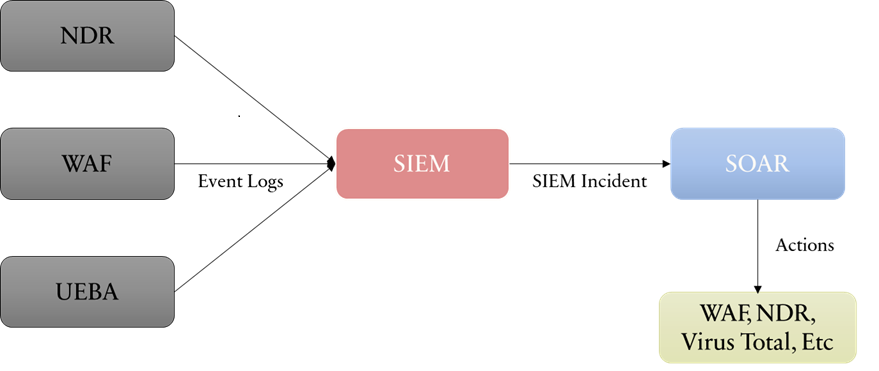
\includegraphics[width=0.9\linewidth]{images/data_flow_soc.png}
    \caption{Data Flow in Security Operations Center (SOC)}
    \label{fig:data-flow-soc}
\end{figure}

All the data collected from these systems is funneled into the \textbf{Security Information and Event Management (SIEM)} platform. The SIEM is responsible for aggregating logs, normalizing event data, correlating security events, and identifying potential incidents. It applies correlation rules and heuristics to generate alerts based on suspicious activities or known indicators of compromise. The SIEM serves as the central hub for visibility and detection across the SOC.

These alerts, along with the enriched context from the SIEM, are then forwarded to the \textbf{Security Orchestration, Automation, and Response (SOAR)} platform:

\begin{itemize}[itemsep=0pt,parsep=0pt,topsep=0pt,partopsep=0pt]
    \item \textbf{SOAR}: Automates the triage and response process using predefined playbooks and workflows. It orchestrates actions across tools, facilitates enrichment (e.g., IP reputation checks), and enables both automated and manual responses.
\end{itemize}

As part of its enrichment process or during automated remediation, the SOAR platform may communicate with additional tools and services:

\begin{itemize}[itemsep=0pt,parsep=0pt,topsep=0pt,partopsep=0pt]
    \item \textbf{Threat Intelligence (e.g., VirusTotal)}: Provides contextual data about IP addresses, domains, file hashes, and URLs to enhance detection and validate alerts.
    \item \textbf{Internal Tools (e.g., WAF, NDR)}: Used during automated response to isolate endpoints, block malicious traffic, or escalate incidents.
\end{itemize}

Finally, the SOAR platform generates a structured response, which may include a combination of automated actions and manual analyst decisions. The entire flow—from data collection to response—is tracked and logged to support auditing, compliance, and continuous improvement of SOC workflows.

\section{Security Information and Event Management (SIEM) in SOC}

A fundamental component of any Security Operations Center (SOC) is the \textbf{Security Information and Event Management (SIEM)} system, which serves as the data aggregation and correlation backbone of cybersecurity monitoring. SIEM platforms collect and analyze log data from across an organization’s digital infrastructure, including endpoints, servers, network devices, firewalls, intrusion detection systems, cloud services, and applications. The primary purpose of a SIEM is to provide \textit{real-time visibility into potential security threats} by aggregating disparate security logs, normalizing them, applying correlation rules, and generating alerts for further investigation by SOC analysts. According to Microsoft~\cite{microsoftsiem}, SIEM solutions are designed to help security teams detect attacks early, prioritize incidents, and comply with regulatory requirements by maintaining detailed audit trails and forensic data.

In a typical SOC workflow, the SIEM acts as the \textit{initial source of alert generation}. It uses pre-defined correlation rules, statistical models, and sometimes machine learning to detect anomalies such as unusual user behavior, suspicious login patterns, or known indicators of compromise (IoCs). These alerts are then triaged by analysts who decide whether they represent true threats or false positives. Leading SIEM tools such as IBM QRadar, Splunk Enterprise Security, Microsoft Sentinel, and ArcSight offer customizable dashboards, threat detection use-cases, and built-in compliance reporting, making them well-suited to both enterprise and government cybersecurity needs.

One key distinction to understand is the difference between \textbf{SIEM and SOAR}, as both platforms are often used in conjunction within a SOC. While SIEM systems focus on \textit{data collection, aggregation, and detection}, SOAR platforms concentrate on \textit{response orchestration, automation, and workflow execution}. SIEM is passive in that it alerts security teams to potential incidents; SOAR is active in that it can automatically take predefined actions—such as blocking an IP, sending notifications, or initiating a playbook—based on the data SIEM provides. As noted by Palo Alto Networks~\cite{paloalto}, SIEM answers the ``what happened?'' and ``where did it happen?'' questions, while SOAR answers ``what do we do about it?''

Furthermore, SIEM solutions typically operate at \textit{higher data volumes}, integrating with a wide array of systems and often ingesting terabytes of log data daily. This massive volume makes SIEMs excellent for \textit{long-term log retention and forensic investigations}, especially in regulated industries. However, this data-centric approach also leads to challenges such as \textit{alert fatigue} and \textit{false positives}, which SOAR platforms are designed to alleviate through automated triage, enrichment, and decision-making. As Gartner highlights, modern SOCs should not treat SIEM and SOAR as competing solutions, but rather as \textit{complementary systems} that, when integrated, can significantly improve the overall efficiency and responsiveness of cybersecurity operations~\cite{gartner-siem-soar}.

In summary, SIEM is the eyes and ears of the SOC, providing centralized, real-time detection of security-relevant events across a wide range of digital assets. Its integration with SOAR platforms transforms this visibility into action, enabling scalable, consistent, and intelligent incident response. In high-stakes environments such as defense and national infrastructure, this combination of SIEM for detection and SOAR for orchestration forms the backbone of effective cyber defense.

\begin{table}[H]
\centering
\caption{Comparison of SIEM and SOAR in SOC}
\begin{tabular}{|p{4cm}|p{5cm}|p{5cm}|}
\hline
\textbf{Feature} & \textbf{SIEM (Security Information and Event Management)} & \textbf{SOAR (Security Orchestration, Automation, and Response)} \\
\hline
Primary Function & Aggregates and correlates log data for threat detection & Automates response actions and orchestrates tools \\
\hline
Focus Area & Monitoring, alerting, and data analysis & Incident response, workflow automation, playbook execution \\
\hline
Data Sources & Logs from endpoints, servers, network devices, and applications & Inputs from SIEM, threat intel feeds, manual triggers \\
\hline
Response Capability & Alert generation only (manual response required) & Supports automated and manual responses \\
\hline
Typical Output & Dashboards, correlation alerts, compliance reports & Executed actions, response workflows, status tracking \\
\hline
Alert Handling & Detects and prioritizes alerts; triage is manual & Automates triage, enrichment, and routing \\
\hline
Challenges Addressed & Data visibility, compliance, threat correlation & Alert fatigue, response delays, process inconsistency \\
\hline
\end{tabular}
\label{tab:siem-vs-soar}
\end{table}

\section{SIEM Incident Flow to SOAR}

One of the most critical integrations within a Security Operations Center (SOC) is the connection between the SIEM and the SOAR platform. This integration enables a seamless transition from \textit{threat detection} (performed by SIEM) to \textit{incident response} (orchestrated by SOAR). A \textbf{SIEM incident} is typically an event or an alert that has been generated based on the correlation of log data received from various security tools such as firewalls, endpoint protection software, network devices, servers, and cloud environments. According to Microsoft~\cite{microsoftsiem}, the SIEM continuously collects and analyzes data from multiple sources, looking for known attack patterns, anomalies, and behavior that matches correlation rules or machine learning models. When such an event is detected, it is flagged as an incident and recorded with a detailed set of metadata.

A typical SIEM incident contains structured fields such as:

\begin{itemize}[itemsep=0pt,parsep=0pt,topsep=0pt,partopsep=0pt]
    \item \textbf{Alert ID}: Unique identifier for the incident or alert.
    \item \textbf{Timestamp}: Time at which the event occurred or was detected.
    \item \textbf{Source IP / Host}: Origin of the suspicious activity.
    \item \textbf{Destination IP / Host}: Targeted system or service.
    \item \textbf{Username}: Account associated with the event (if applicable).
    \item \textbf{Severity Level}: Assigned severity (e.g., low, medium, high, critical).
    \item \textbf{Event Type / Rule Name}: Category or rule that triggered the alert (e.g., brute force, malware, lateral movement).
    \item \textbf{Raw Logs / Correlation Data}: Detailed evidence or event logs that support the detection.
    \item \textbf{Tactic / Technique (if mapped)}: MITRE ATT\&CK classification, if supported.
\end{itemize}

This incident data is then forwarded in real-time or near real-time to the \textbf{Security Orchestration, Automation, and Response (SOAR)} platform via APIs, message queues, or webhooks. As noted by Palo Alto Networks~\cite{paloalto}, the SOAR platform ingests the full context of the incident, enabling rapid enrichment, triage, and action.

Once the incident is received, the SOAR system begins the triage process. It may apply severity filters, check asset criticality, or consult external threat intelligence databases (e.g., VirusTotal, AbuseIPDB) to enrich the incident data. Based on this context, predefined playbooks are triggered. These playbooks can include actions such as:

\begin{itemize}[itemsep=0pt,parsep=0pt,topsep=0pt,partopsep=0pt]
    \item Notifying the responsible analyst or team
    \item Blocking an IP address using a firewall or EDR tool
    \item Isolating a host from the network
    \item Gathering additional context from threat feeds or SIEM
    \item Automatically resolving the alert if it is a known benign pattern
\end{itemize}

Throughout this lifecycle, the SOAR platform maintains a case file containing the timeline of actions, analyst comments, and response outcomes. As Gartner notes, this automation enhances consistency and dramatically reduces the Mean Time to Respond (MTTR), which is critical in large-scale SOC environments~\cite{gartner-siem-soar}.

Thus, the SIEM-to-SOAR pipeline enables SOCs to convert raw detection into intelligent, actionable response while maintaining operational oversight and auditability.
